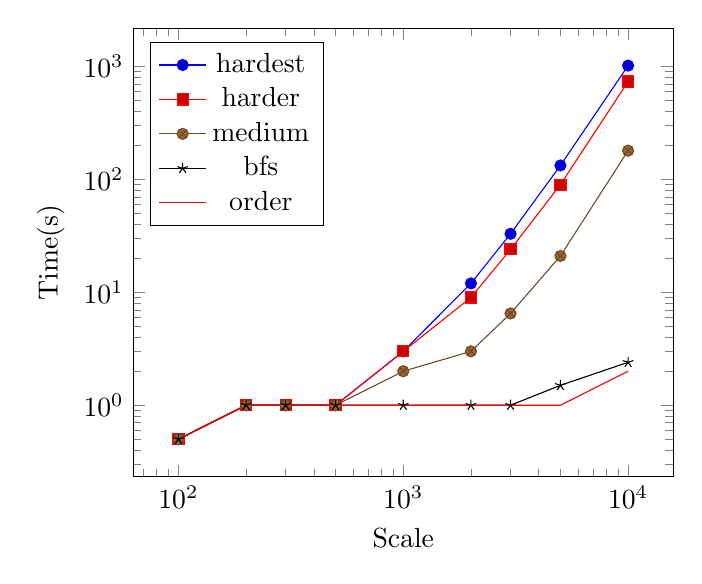
\begin{tikzpicture}
    \pgfplotstableread [row sep=crcr]
    {scale hardest harder medium bfs order\\100 0.5 0.5 0.5 0.5 0.5\\200 1 1 1 1 1\\300 1 1 1 1 1\\500 1 1 1 1 1\\1000 3 3 2 1 1\\2000 12 9 3 1 1\\3000 33 24 6.5 1 1\\5000 133 90 21 1.5 1\\10000 1020 736 180 2.4 2\\\\}
    {\value}
    \begin{loglogaxis}[legend pos=north west,
    ylabel={Time(s)},
    xlabel={Scale},]
     \addplot+ [] table[y=hardest] {\value};
     \addplot+ [] table[y=harder] {\value};
    \addplot+ [] table[y=medium] {\value};
    \addplot+ [] table[y=bfs] {\value};
    \addplot[red] table[y=order] {\value};
    \legend{hardest,harder,medium,bfs,order};
    \end{loglogaxis}
\end{tikzpicture}